\subsection{Rastrigin 2D}

\par Rastrigin is a non-convex function first proposed by Rastrigin as a 2-dimensional function and then generalized later on to multiple dimensions. The function is defined by:

$$
f_4(x) = 20 + x_1^2 - 10 \cos (2 \pi x_1) + x_2^2 - 10 \cos (2 \pi x_2)
$$

It has multiple maxima and minima and its global minima is also at $x=0$.

\par Both functions are tested five times with the Rastrigin 2D function with the same starting random population and a dimensional space of [$-2\pi$, $2\pi$].

\begin{table}[ht]
\scriptsize
\begin{tabular}{l|ccccc}
\textbf{}        & \textbf{Trial 1} & \textbf{Trial 2} & \textbf{Trial 3} & \textbf{Trial 4} & \textbf{Trial 5} \\
\hline
LOA End Fitness  & 0.083296         & 0.022199         & 0.001943         & 0.0015496        & 0.30548          \\
LOA Evaluations  & 3314             & 3513             & 3443             & 3536             & 3496             \\
iLOA End Fitness & 0.00022399       & 0.0015992        & 0.0012708        & 0.40278          & 3.1202E-05       \\
iLOA Evaluations & 2811             & 2767             & 2711             & 2743             & 2894
\end{tabular}
\caption{ \scriptsize LOA vs. iLOA: Rastrigin 2D ($f_4$)}
\end{table}

\begin{figure}
  \centering
  \begin{subfigure}[b]{0.4\textwidth}
    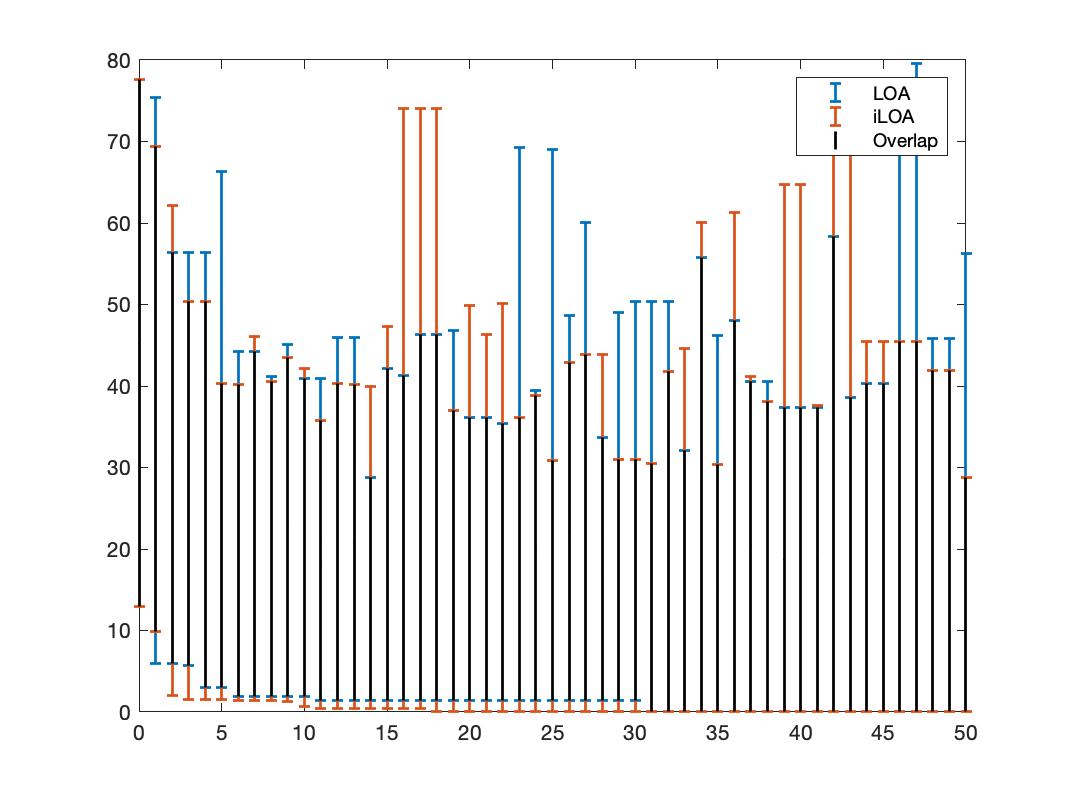
\includegraphics[width=\textwidth]{img/bars/f4/1}
    \caption{ \scriptsize Trial 1: Fitness Range (y) over Iterations (x)}
    \label{fig:f4-b-1}
  \end{subfigure}
  \begin{subfigure}[b]{0.4\textwidth}
    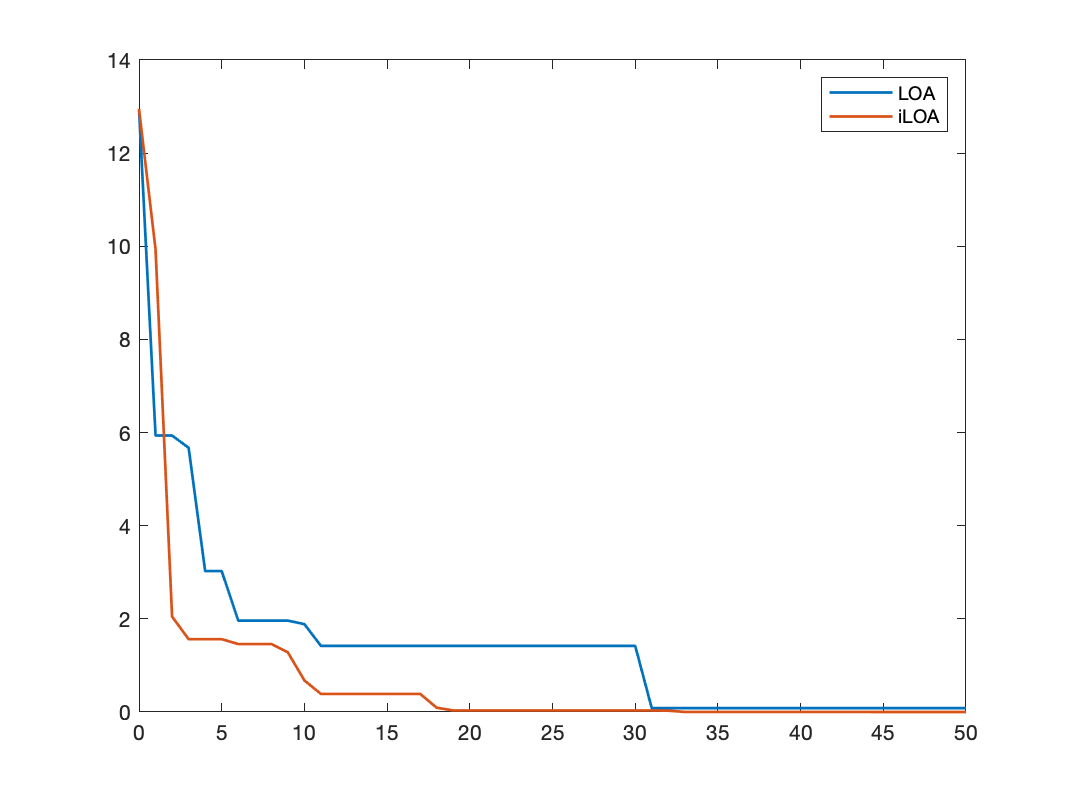
\includegraphics[width=\textwidth]{img/fits/f4/1}
    \caption{ \scriptsize Trial 1: Minimum Fitness (y) over Iterations (x)}
    \label{fig:f4-f-1}
  \end{subfigure}

  \begin{subfigure}[b]{0.4\textwidth}
    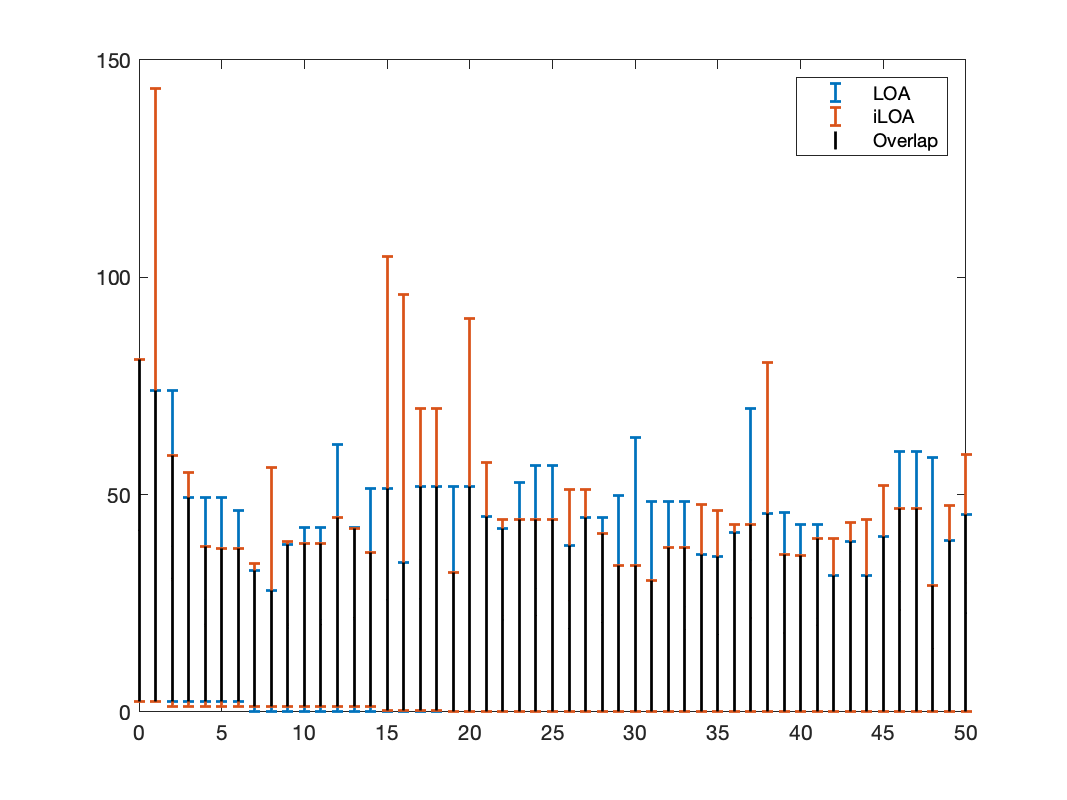
\includegraphics[width=\textwidth]{img/bars/f4/2}
    \caption{ \scriptsize Trial 2: Fitness Range (y) over Iterations (x)}
    \label{fig:f4-b-2}
  \end{subfigure}
  \begin{subfigure}[b]{0.4\textwidth}
    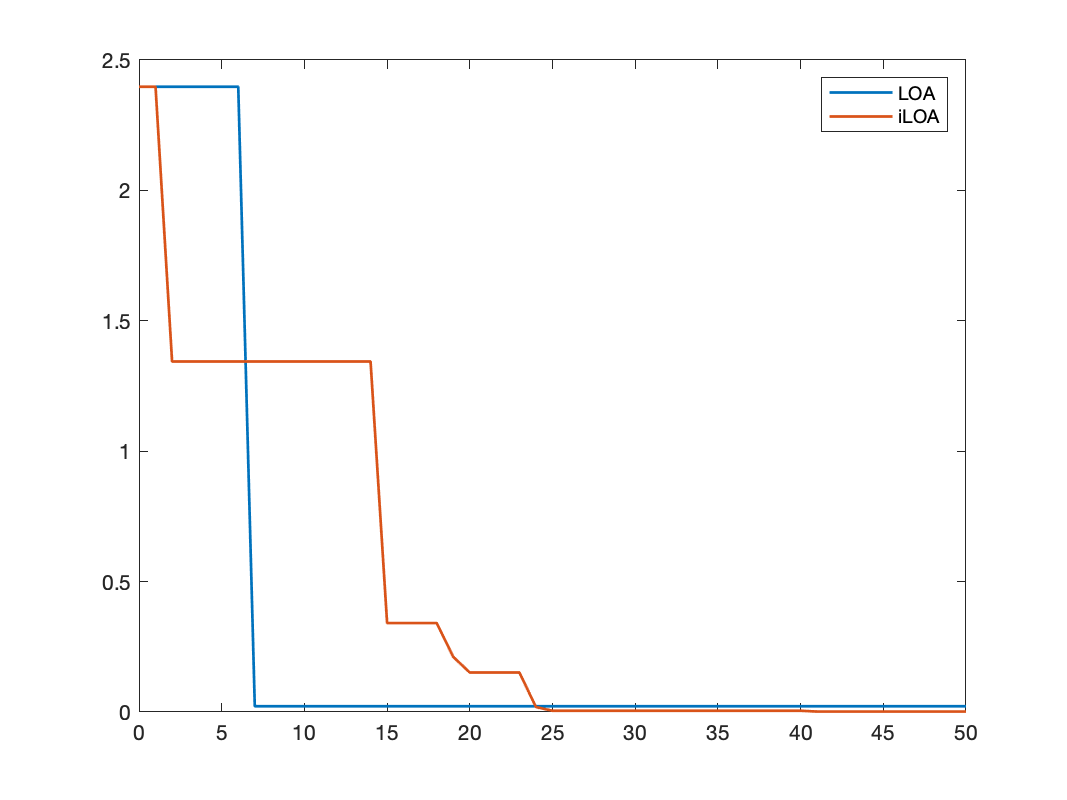
\includegraphics[width=\textwidth]{img/fits/f4/2}
    \caption{ \scriptsize Trial 2: Minimum Fitness (y) over Iterations (x)}
    \label{fig:f4-f-2}
  \end{subfigure}

  \begin{subfigure}[b]{0.4\textwidth}
    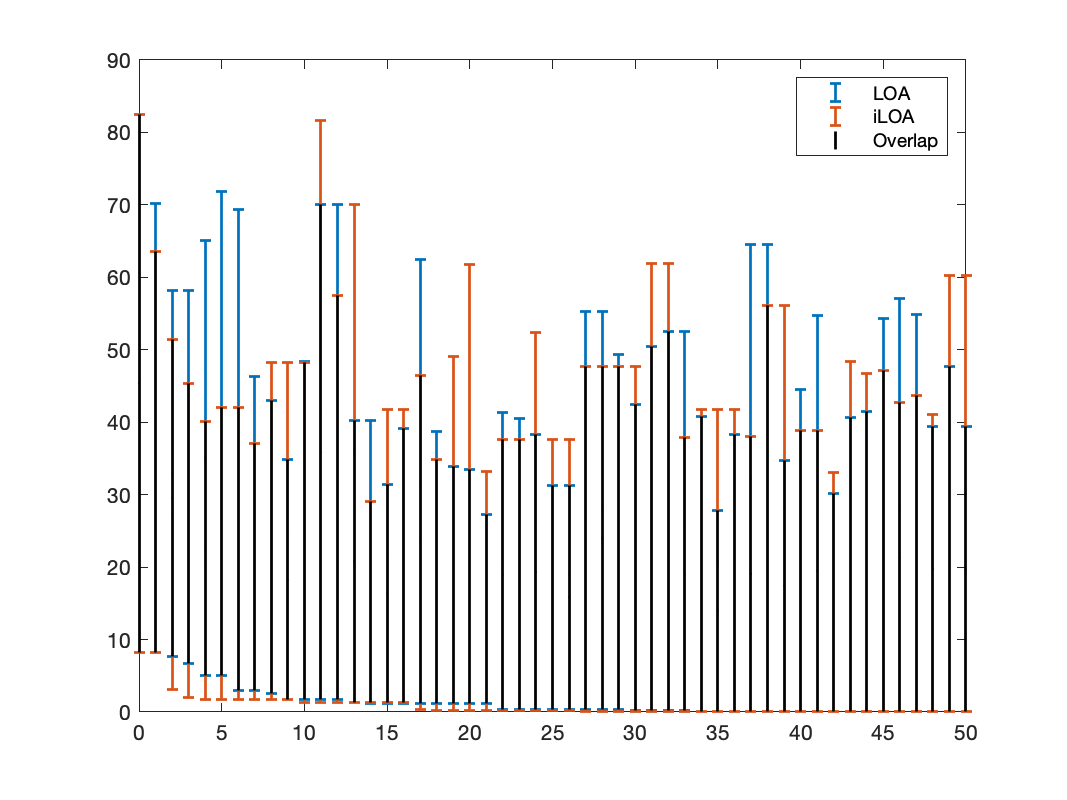
\includegraphics[width=\textwidth]{img/bars/f4/3}
    \caption{ \scriptsize Trial 3: Fitness Range (y) over Iterations (x)}
    \label{fig:f4-b-3}
  \end{subfigure}
  \begin{subfigure}[b]{0.4\textwidth}
    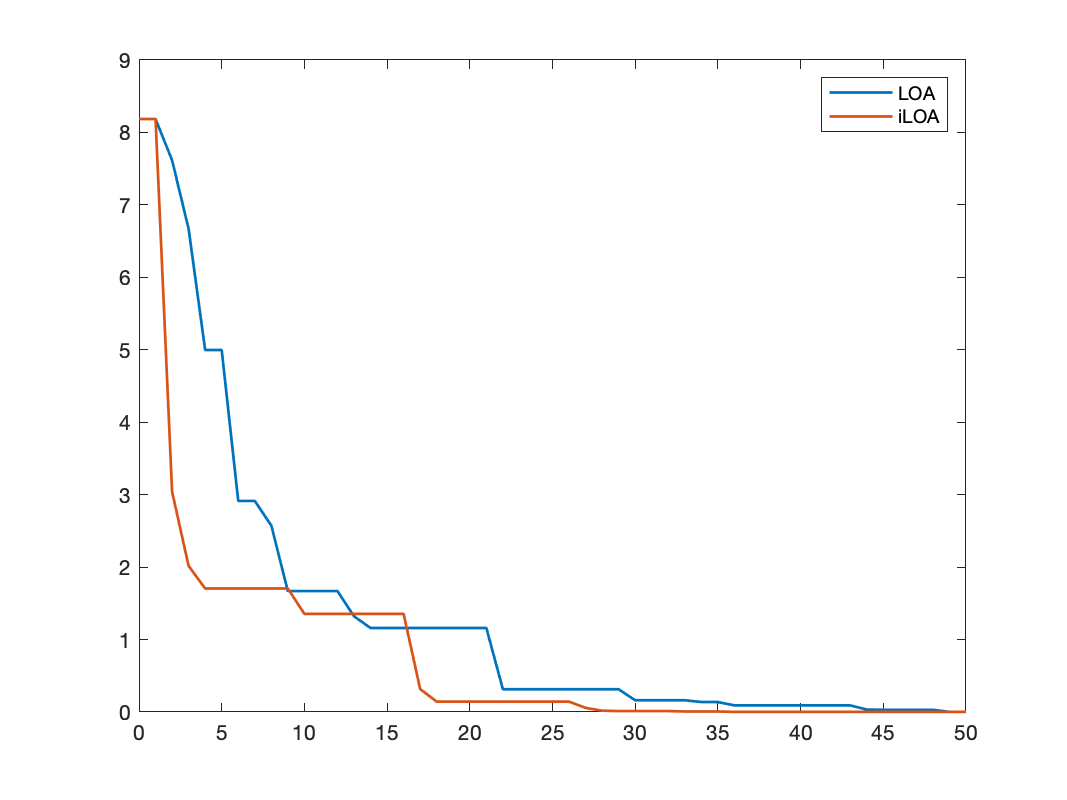
\includegraphics[width=\textwidth]{img/fits/f4/3}
    \caption{ \scriptsize Trial 3: Minimum Fitness (y) over Iterations (x)}
    \label{fig:f4-f-3}
  \end{subfigure}

  \begin{subfigure}[b]{0.4\textwidth}
    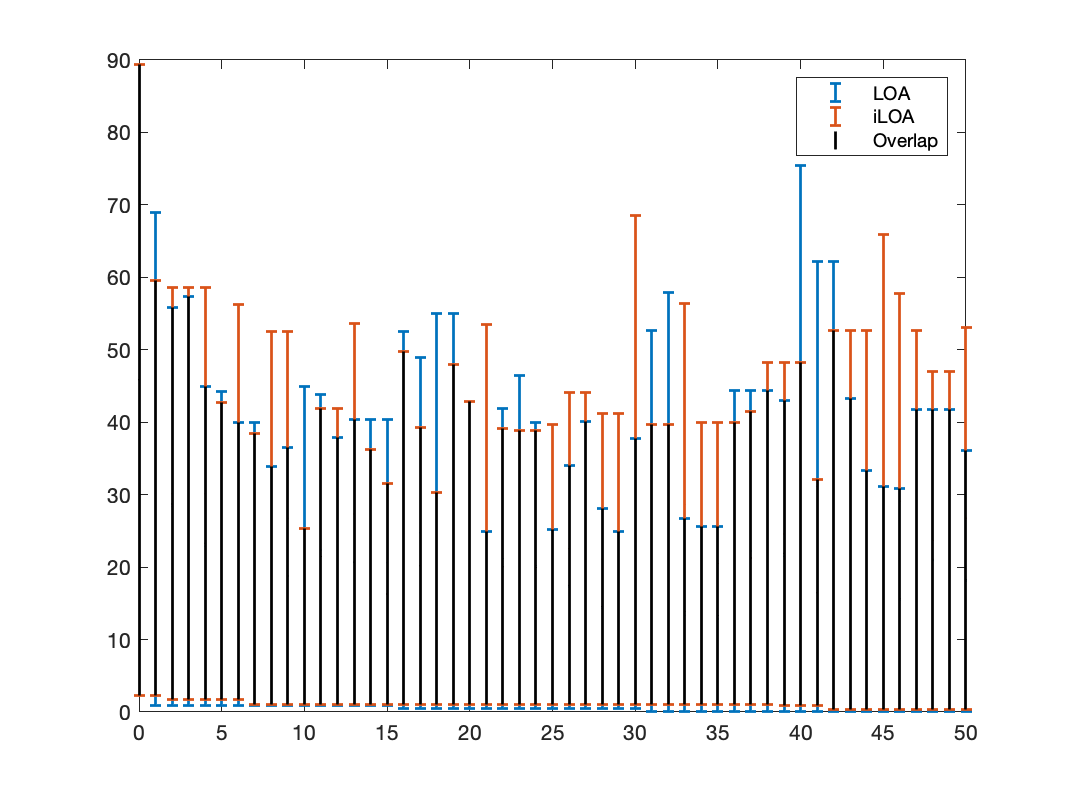
\includegraphics[width=\textwidth]{img/bars/f4/4}
    \caption{ \scriptsize Trial 4: Fitness Range (y) over Iterations (x)}
    \label{fig:f4-b-4}
  \end{subfigure}
  \begin{subfigure}[b]{0.4\textwidth}
    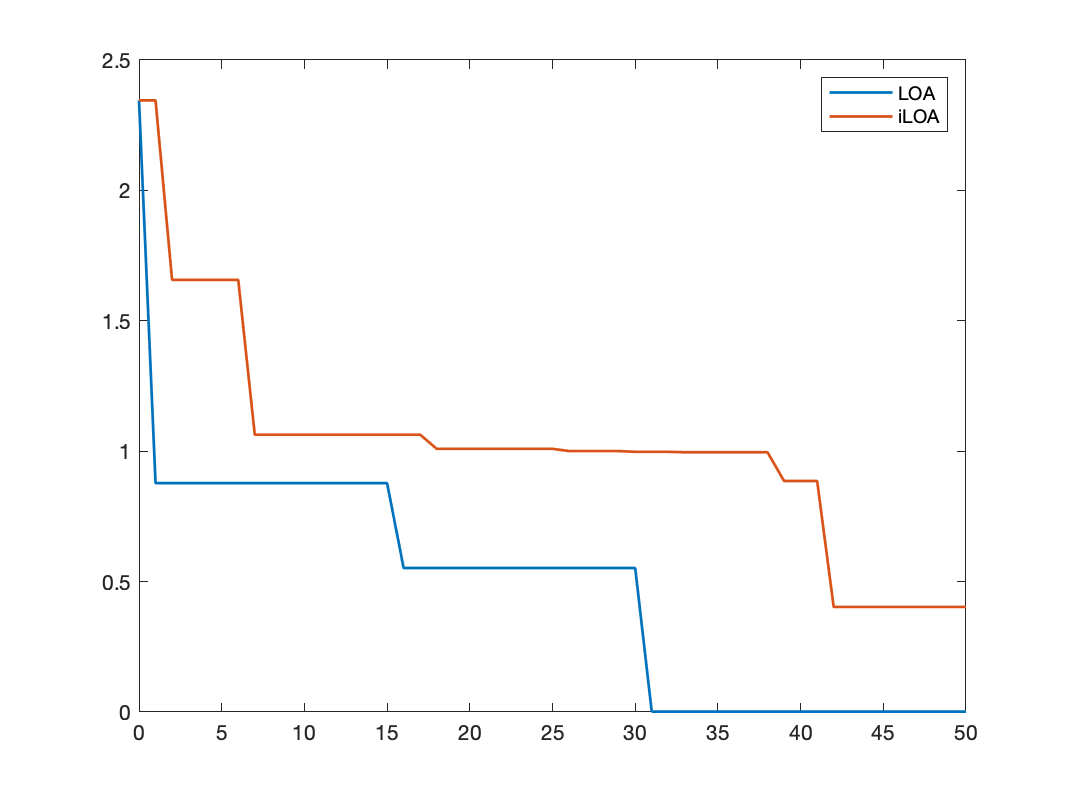
\includegraphics[width=\textwidth]{img/fits/f4/4}
    \caption{ \scriptsize Trial 4: Minimum Fitness (y) over Iterations (x)}
    \label{fig:f4-f-4}
  \end{subfigure}

  \begin{subfigure}[b]{0.4\textwidth}
    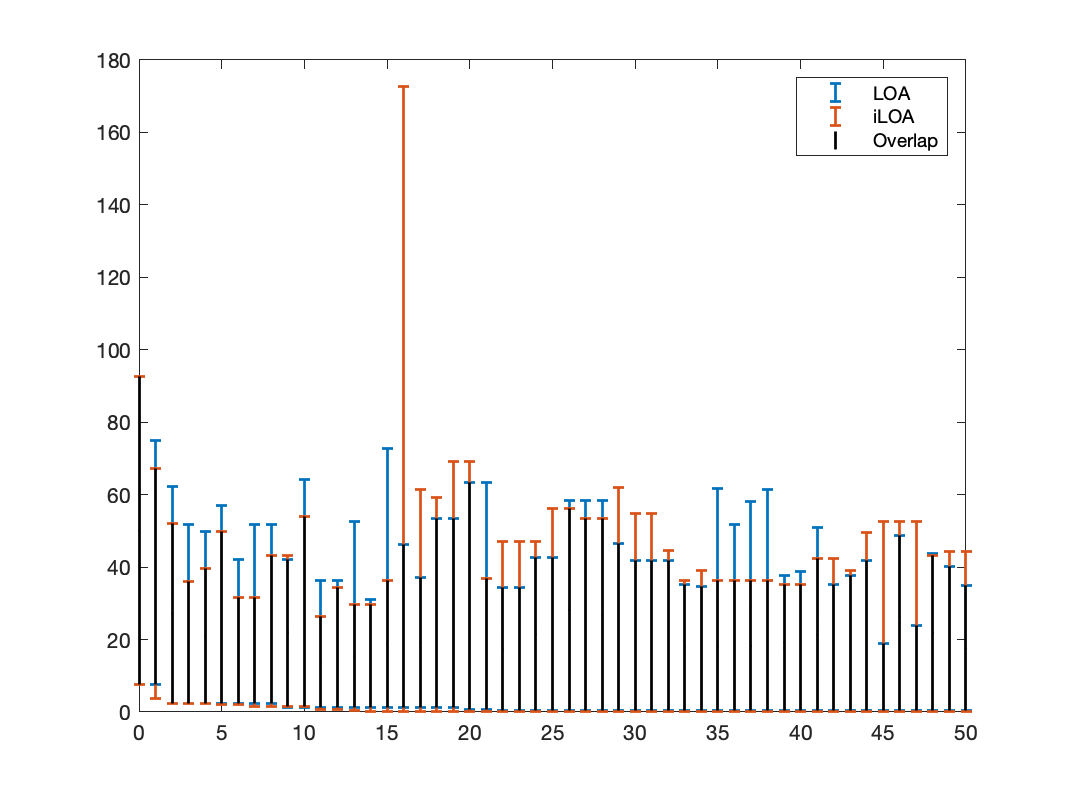
\includegraphics[width=\textwidth]{img/bars/f4/5}
    \caption{ \scriptsize Trial 5: Fitness Range (y) over Iterations (x)}
    \label{fig:f4-b-5}
  \end{subfigure}
  \begin{subfigure}[b]{0.4\textwidth}
    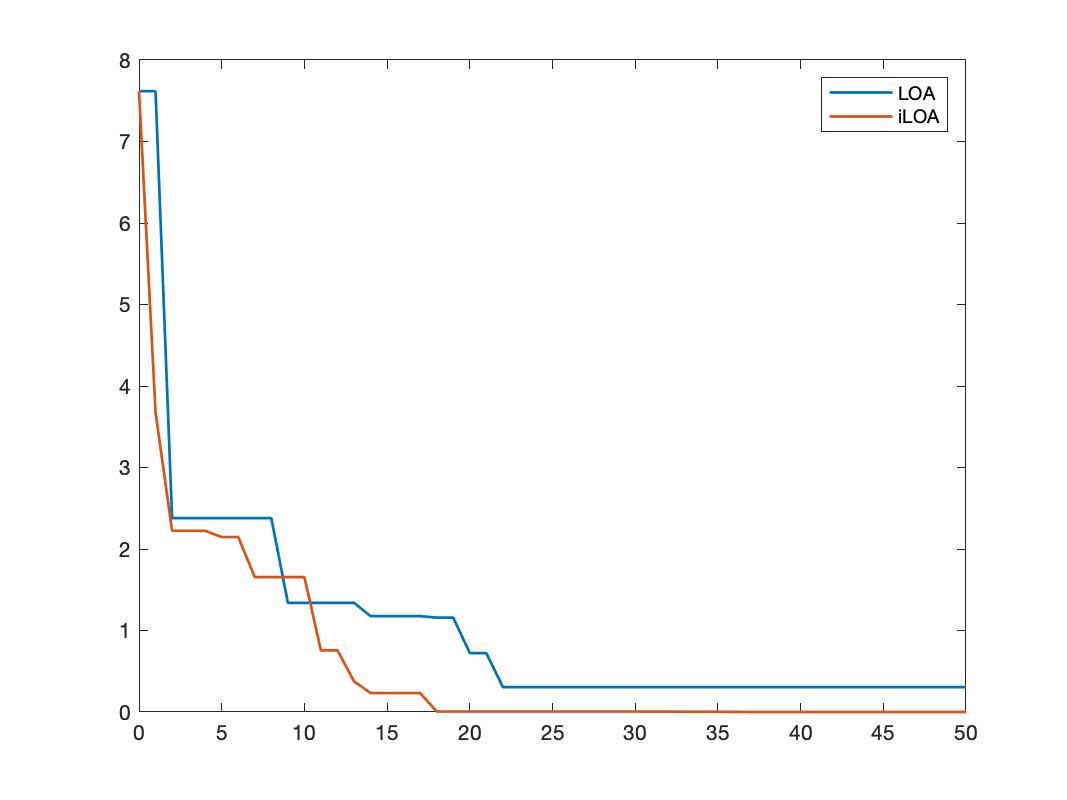
\includegraphics[width=\textwidth]{img/fits/f4/5}
    \caption{ \scriptsize Trial 5: Minimum Fitness (y) over Iterations (x)}
    \label{fig:f4-f-5}
  \end{subfigure}

  \caption{ \scriptsize LOA vs. iLOA: Rastrigin 2D ($f_4$)}
\end{figure}
